\documentclass[border=3pt]{standalone}
\usepackage{xcolor}
\usepackage{tikz}
\usetikzlibrary{arrows.meta,decorations.pathreplacing,positioning}

\definecolor{flowblue}{HTML}{2563EB}
\definecolor{flowgreen}{HTML}{059669}
\definecolor{flowink}{HTML}{1E293B}

\begin{document}
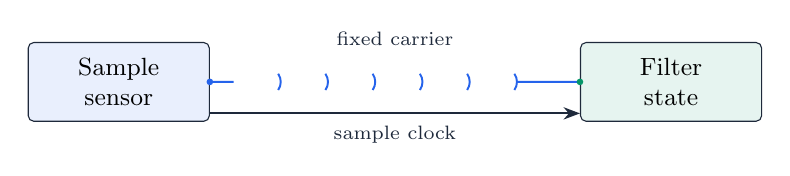
\begin{tikzpicture}[
  >=Stealth,
  block/.style={draw=flowink,rounded corners=2pt,minimum width=2.3cm,
    minimum height=1cm,align=center,font=\small},
  label/.style={font=\scriptsize,text=flowink,fill=white,inner sep=1.5pt}
]
  \node[block,fill=flowblue!10] (sample) {Sample\\sensor};
  \node[block,fill=flowgreen!10,right=4.7cm of sample] (filter) {Filter\\state};

  \draw[flowblue,line width=.7pt,decorate,
    decoration={waves,segment length=6mm,radius=1.8mm,angle=35,
      pre length=3mm,post length=5mm}]
    (sample.east) -- node[label,above=4mm] {fixed carrier} (filter.west);
  \draw[-Stealth,flowink,line width=.65pt]
    ([yshift=-4mm]sample.east) -- node[label,below=1mm] {sample clock}
    ([yshift=-4mm]filter.west);

  \fill[flowblue] (sample.east) circle (1.2pt);
  \fill[flowgreen] (filter.west) circle (1.2pt);
\end{tikzpicture}
\end{document}
